% 2.2
% Higgs Mechanism

In the standard model the $W^{\pm}$ and $Z$ bosons are massive but the photon is massless.
Since gauge invariance dictates that a mass term is forbidden in the Lagrangian, this seems to pose a problem.
Disaster is averted because $SU(2)_W \times U(1)_Y$ is spontaneously broken to $U(1)_{EM}$.
In the standard model this is accomplished by adding a complex scalar doublet field to the theory.
The field is named the Higgs field after one of its discoverers.
The following discussion shows how electroweak symmetry breaking is facilitated by the Higgs \cite{Quigg:ds52, Quigg:ds53, peskin:book}.

Lets introduce a complex elementary scalar doublet $\Phi=\left(\begin{matrix}\phi^+\\\phi_0\end{matrix}\right)$ that transforms in the (1,2,$\frac{1}{2}$) representation of $SU(3)_C\times SU(2)_L\times U(1)_Y$.
We allow all terms in the Lagrangian that have mass dimension $\leq 4$, thus ignoring irrelevant operators,
\begin{equation}
  \Lagr_H=(D_\mu\Phi)^\dagger(D^\mu\Phi)+\mu^2\Phi^\dagger\Phi-|\lambda|(\Phi^\dagger\Phi)^2,
\end{equation}
with covariant derivative
\begin{equation}
  D_\mu\Phi=(\partial_\mu-igA^a_\mu\tau^a-ig'YB_\mu)\Phi.
\end{equation}
$A^a_\mu$ and $B_\mu$ are the $SU(2)$ and $U(1)$ gauge bosons respectively.
The coupling constant $g$ belongs to $SU(2)$ and the coupling constant $g'$ belongs to $U(1)$.
Finally $Y$ is the generator of hypercharge, $\tau^a$ are the generators of $SU(2)$ and are related to the Pauli matrices
\begin{equation}
  \tau^a=\frac{1}{2}\sigma^a.
\end{equation}

We can now identify the potential $V(\Phi)$ as
\begin{equation}
  V(\Phi)=-\mu^2\Phi^\dagger\Phi+|\lambda|(\Phi^\dagger\Phi)^2,
\end{equation}
this potential is shown in figure \ref{fig:higgspot}.
As long as $\mu^2$ is positive the potential has a spontaneously broken symmetry.
Gauge invariance allows us to choose the vacuum state to correspond to the vacuum expectation value (VEV)
\begin{equation}
  \left<\Phi\right>_0=\frac{\nu}{\sqrt{2}}\left(\begin{matrix}0 \\ \nu\end{matrix}\right),
\end{equation}
where $\nu=\sqrt{\frac{\mu^2}{|\lambda|}}$.
Moreover, $\nu$ is related to the Fermi constant, $G_F$, by
\begin{equation}
  \nu=\frac{1}{2^{1/4}\sqrt{G_F}}\approx 246 \mbox{ GeV}.
\end{equation}

\begin{figure}[h]
  \begin{center}
    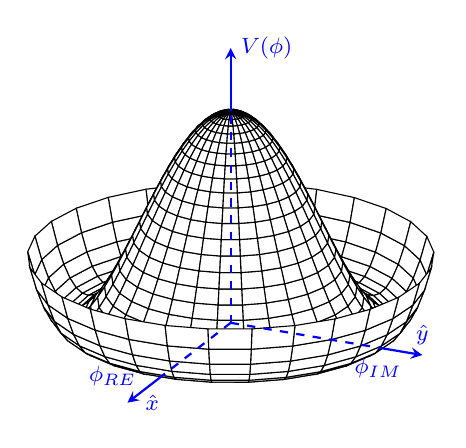
\begin{tikzpicture}
        \begin{axis}[
            hide axis,
            %axis lines=middle,
%            axis on top,
%            axis line style={blue,dashed,thick},
%            ymin=-2,ymax=2,
%            xmin=-2,xmax=2,
%            zmin=-2,zmax=2,
            samples=30,
            domain=0:360,
            y domain=0:1.25,clip=false
        ]
        \addplot3 [surf, shader=flat, draw=black, fill=white, z buffer=sort]
           ({sin(x)*y}, {cos(x)*y}, {(y^2-1)^2});
        \draw[blue,thick,dashed] (axis cs:0,0,0) -- (axis cs:1,0,0)
                    node[below,font=\footnotesize]{$\phi_{\text{IM}}$};
        \draw[blue,thick,-stealth] (axis cs:1,0,0) -- (axis cs:1.3,0,0)
                    node[above,font=\footnotesize]{$\hat{y}$};
        \draw[blue,thick,dashed] (axis cs:0,0,0) -- (axis cs:0,-1,0)
                    node[left=2mm,font=\footnotesize]{$\phi_{\text{RE}}$};
        \draw[blue,thick,-stealth] (axis cs:0,-1,0) -- (axis cs:0,-1.5,0)
                    node[right=1mm,font=\footnotesize]{$\hat{x}$};
        \draw[blue,thick,dashed] (axis cs:0,0,0) -- (axis cs:0,0,1)
                    %node[left=2mm,font=\footnotesize]{$\phi_{\text{RE}}$}
                    ;
        \draw[blue,thick,-stealth] (axis cs:0,0,1) -- (axis cs:0,0,1.3)
        node[right,font=\footnotesize]{$V(\phi)$};
        \end{axis}
    \end{tikzpicture}
  \end{center}
  \caption{The Higgs potential with $\mu^2>0$ has a spontaneously broken global symmetry.  We can think of this classically. The origin is a local maximum of potential energy and therefore an unstable equilibrium. If we place a particle at the origin any perturbation will push the particle `down hill' to a minimum of the potential.  Since there are a number of degenerate minima, choosing one spontaneously breaks the symmetry.}
  \label{fig:higgspot}
\end{figure}


If we assign our theory to have hypercharge $Y=+\frac{1}{2}$, a complete gauge transformation in this theory is
\begin{equation}
  \Phi\rightarrow e^{i\alpha^a(x)\tau^a}e^{i\beta(x)/2}\Phi.
\end{equation}
Making the particluar choice of $\alpha^1=\alpha^2=0$ and $\alpha^3=\beta$ we see that $\left<\Phi\right>$ is invariant.
Therefore the theory still contains an unbroken U(1) symmetry which we identify with electromagnetism.
This unbroken U(1) symmetry contains one massless gauge boson which is the photon.
The other three gauge bosons corresponding to the broken generators of the symmetry group become massive.
The massive gauge bosons get their mass from the square of the kinetic term evaluated at the VEV
\begin{equation}
  (D_\mu\Phi)^\dagger(D^\mu\Phi)=\frac{1}{2}(\begin{matrix}0& \nu\end{matrix})\Big(gA^a_\mu\tau^a+\frac{1}{2}g'B_\mu\Big)\Big(gA^{b\mu}\tau^\mu+\frac{1}{2}g'B^\mu\Big)\left(\begin{matrix}0\\\nu\end{matrix}\right).
\end{equation}
Substituting $\tau^a$ and taking the product we get
\begin{equation}
  (D_\mu\Phi)^\dagger(D^\mu\Phi)=\frac{\nu^2}{8}\Big[g^2(A^1_\mu)^2+g^2(A^2_\mu)^2+(-gA^3_\mu+g'B_\mu)^2\Big].
\end{equation}
We can now perform a field redefinition and recover
\begin{align}
  W^\pm_\mu&=\frac{1}{\sqrt{2}}\Big(A^1_\mu\mp A^2_\mu\Big)&\mbox{\quad with mass\quad} m_W=g\frac{\nu}{2}\\
  Z_\mu&=\frac{1}{\sqrt{g^2+g'^2}}\Big(gA^3_\mu-g'B_\mu\Big)&\mbox{\quad with mass\quad} m_Z=\sqrt{g^2+g'^2}\frac{\nu}{2}\\
  A_\mu&=\frac{1}{\sqrt{g^2+g'^2}}\Big(g'A^3_\mu+gB_\mu\Big)&\mbox{\quad with mass\quad} m_A=0,
\end{align}
which are the standard model $W^\pm, Z$ bosons and photon.

The change in basis from the original massless bosons to massive bosons and photon is characterized by the weak mixing angle $\theta_w$:
\begin{equation}
  \left(\begin{matrix}Z_\mu\\A_\mu\end{matrix}\right)=\left(\begin{matrix}\cos\theta_w & -\sin\theta_w\\\sin\theta_w & \cos\theta_w\end{matrix}\right)\left(\begin{matrix}A^3_\mu\\ B_\mu\end{matrix}\right),
\end{equation}
with
\begin{equation}
  \cos\theta_w=\frac{g}{\sqrt{g^2+g'^2}},\quad\sin\theta_w=\frac{g'}{\sqrt{g^2+g'^2}}.
\end{equation}

When the $W^\pm$ and $Z$ bosons become massive they each gain an additional longitudinal degree of freedom.
These new degrees of freedom aren't free; they come from the three components of the Higgs doublet $\Phi$ associated with the original broken symmetry.
The Goldstone mechanism facilitates this transfer of degrees of freedom.
The vernacular is that the massless Goldstone bosons of the original theory are ``eaten" by the $W^\pm$ and $Z$.


Additionally, the Higgs mechanism provides a mass for the standard model fermions.
Fermion mass terms are forbidden in the standard model because they would violate local gauge invariance since left and right fermions transform differently.
Now that we have a scalar field $\Phi$ we can couple it to our fermion with a Yukawa coupling, $-c\bar{f_L}\Phi f_R$.
In such a term $f_L$ and $f_R$ are the right and left components of the fermion, $c$ is an arbitrary coupling characterizing the strength of the interaction with the Higgs VEV, and $\Phi$ is the Higgs VEV.
Heavy particles like the top have a large value of $c$ while light particles like the up quark have a small value of $c$.

Finally, the Higgs Boson, a particle excitations of the Higgs field, was recently discovered at the Large Hadron Collider (LHC).The discovery was announced to the pulbic July 4, 2012.
Current experimental results pin the Higgs mass at 126 GeV.
Peter Higgs and François Englert shared the Nobel prize in 2013 for their work in developing the theory of EWSB through the Higgs mechanism.
